\chapter{Systemmodelle}
\section{Anwendungsfälle}
\subsection{Bedienung der Android App}
\begin{center}
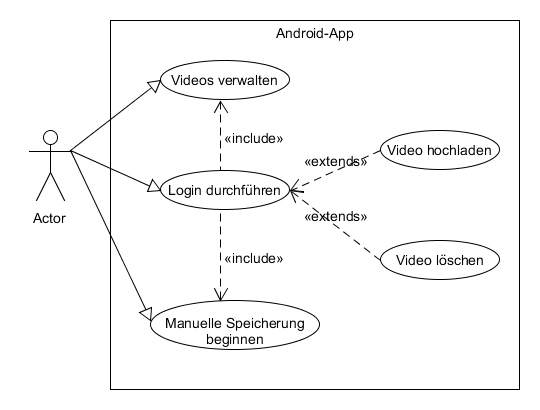
\includegraphics[width=1\textwidth]{subtopicsFuncspec/systemModels/App-AFD-UML.png}
\end{center}
Dieser Anwendungsfall beschreibt die Bedienung der App. 
Der Benutzer kann hierbei mehrere Aktionen ausführen:
\begin{itemize}
\item Login durchführen
\item Videos verwalten
\item Den Status setzen
\item Manuelle Speicherung beginnen
\end{itemize}
Um auf alle Funktionen zugreifen zu können muss sich der Benutzer zunächst auf der App einloggen. 
Wenn der Benutzer sein aufgenommenes Videomaterial verwalten will kann er zum einen die Videos auf den Web-Service hochladen oder die Videos löschen.
Des weiteren kann er den Status der "Aufnahme" auf aktiv/inaktiv setzen. Bei aktiv ist der Ringpuffer angeschaltet. 
Außerdem kann man einen manuellen Speichervorgang ohne des Auslösen des Sensors beginnen um zum Beispiel.

\subsection{Bedienung der Website}
\begin{center}
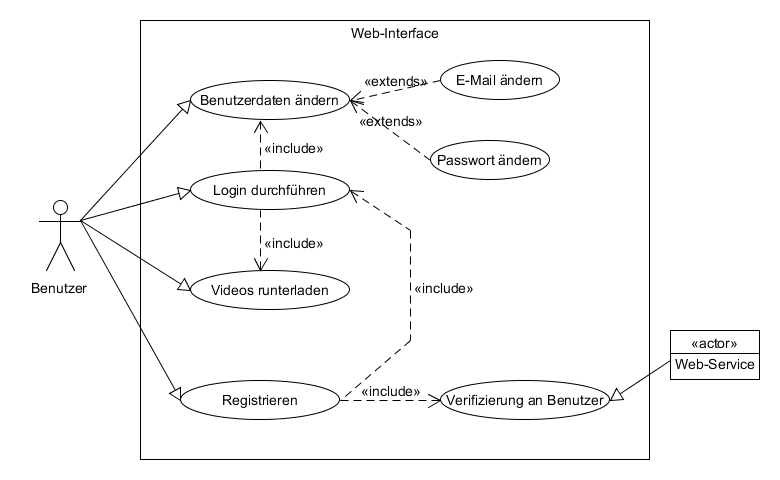
\includegraphics[width=1\textwidth]{subtopicsFuncspec/systemModels/WebsiteAWFDiagram.png}
\end{center}	
Dieser Anwendungsfall beschreibt die Bedienung der Website.
Der Benutzer kann hierbei mehrere Aktionen ausführen:
\begin{itemize}
\item Login durchführen
\item Registrieren
\item Benutzerdaten ändern
\item Videodaten runterladen
\end{itemize}
Um den Service der App und der Website zu nutzen muss sich der Benutzer zu Beginn mit seinen Benutzerdaten registrieren. 
Nun kann er den Login auf der Website oder App durchführen um die Funktionen beider Applikationen zu nutzen. 
Ist der Benutzer eingeloggt kann er seine Benutzerdaten ändern und bereits hochgeladene Videodaten nach der Anonymisierung runterladen.
Nach der Registrierung und Änderung von Benutzerdaten schickt der Web-Service eine Verifizierungs-E-Mail an den Benutzer.
\subsection{Von Appstart bis Videofreigabe}
\begin{center}
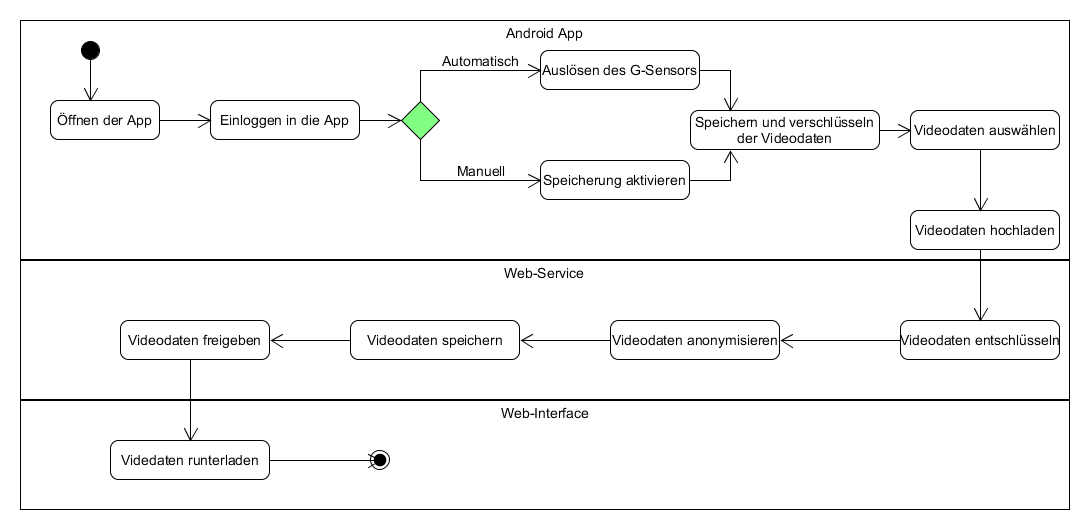
\includegraphics[width=1\textwidth]{subtopicsFuncspec/systemModels/AKDiagramm.png}
\end{center}
Dieses Aktivitätsdiagramm beschreibt den Ablauf vom Start der App bis zur Freigabe und dem Runterladen der Videodaten. 
\begin{enumerate}
\item Öffnen der Applikation
\item Einloggen in die Applikation
\begin{description}
\item Der Benutzer loggt sich mit seinen Anmeldedaten in die Applikation ein um die Funktionen zu nutzen.
\end{description}
\item Automatische oder Manuelle Speicherung
\begin{enumerate}
\item Auslösen des G-Senors
\begin{description}
\item Der G-Sensor löst aus da er einen bestimmten Richtwert überschritten hat und somit beginnt die Speicherung der Videodaten. 
\end{description}
\item Manuelle Speicherung aktivieren
\begin{description}
\item Der Benutzer hat eine manuelle Speicherung angefordert und die Daten werden persistiert.
\end{description}
\end{enumerate}
\item Speichern und verschlüsseln der Videodaten
\begin{description}
\item Bei Beendigung der Aufnahme wird die Videodaten gespeichert und daraufhin mit einer Verschlüsselung versehen.
\end{description}
\item Videodaten auswählen
\item Videodaten hochladen
\begin{description}
\item Die ausgewählte Videodaten wird auf den Web-Service hochgeladen.
\end{description}
\item Videodaten entschlüsseln
\item Videodaten anonymisieren
\begin{description}
\item Nach der Entschlüsselung der Videodaten kann der Web-Service mit der Anonymisierung der Daten beginnen. 
\end{description}
\item Videodaten speichern
\item Videodaten freigeben
\begin{description}
\item Die Videodaten werden auf der Web-Interface zugänglich gemacht.
\end{description}
\item Videodaten runterladen
\begin{description}
\item Nun kann der Benutzer sich einloggen und die Videodaten herunterladen.
\end{description}
\end{enumerate}